%!TEX root = ../main.tex
%
% 磁場
%


\section{磁場の性質}

\subsection{磁石と磁場}

私達の身の周りでは、多くの磁石が使われています。これらの磁石には、大きく分けて、永久磁石と電磁石という2種類があり、常に磁石の性質を持っているものを永久磁石、電流を流したときだけ磁石になるようなものを電磁石といいます。

棒状の永久磁石の重心のところを糸でつるすと、地磁気の方向を向くことが知られて
います。この棒磁石に鉄粉をふりかけると、両端に多く鉄粉が吸い付くことがわかります。この両端を{\bf 磁極}と呼び、北を指す方の磁極を{\bf N極}、南を指す磁極を{\bf S極}と呼びます。これらの磁極間には力が働きますが、これは、一方の磁極が周囲に{\bf 磁場(磁界)}を作り、もう一方の磁極がその磁場を感じるためである、と考えることができます。このような解釈するのが場という概念を用いた考え方です。

磁場の向きは、磁力線(N極から出てS極へ向かう曲線)によって示され、磁場の強さはその「磁力線の密度」=磁束密度によって表すことができます。磁束密度の単位としては、[gauss](ガウス)や[T](テスラ)などが用いられています。

%\paragraph{問題1:}
%鉄が磁石に引きつけられることはよく知られています。では、鉄以外の物は、
%磁石に対してどのように反応するでしょうか。考えてみましょう。
%
%\paragraph{問題2:}
%永久磁石を使った方が便利な場合と、電磁石を使った方が便利な場合をそれ 
%ぞれ考えてみましょう。

\subsection{磁気ヒステリシス曲線}

\begin{wrapfigure}[16]{r}{7cm}
\vspace*{-0.8cm}
\begin{center}
\includegraphics[scale=0.3]{06_Magnetism/MagneticDomain.eps}\\
強磁性体中の磁区\\
\vspace*{0.5cm}
\includegraphics[scale=0.5]{06_Magnetism/hysteresis.eps}\\
磁気ヒステリシス曲線
\end{center}
\end{wrapfigure}


外部の磁場によって磁気を持ち、磁石になる鉄、ニッケル、コバルトなどの金属を{\bf 強磁性体}と呼びます。
強磁性体の内部は小さな磁石の集合体(磁区)でできていて、外部から磁場を与えると徐々に磁区の磁気の方向が外部の磁場の方向にそろうようになり、
全体として磁気を帯びて磁石になります。外部の磁場を強くしていくと磁石の強さ(磁束密度)もそれに応じて強くなりますが、磁区の方向が
全てそろってしまうと磁束密度の大きさは限界に達します。これを{\bf 飽和磁束密度}といい、その強磁性体を用いた
電磁石の最大の強さとなります。

はじめに磁区の方向がバラバラで全体として磁気を持っていなくても、外部の磁場を一度与えて軸の方向をそろえると、外部の磁場をなくしても
強磁性体には磁気が残ります。この時の磁束密度を{\bf 残留磁束密度}といい、強磁性体を使った永久磁石の強さとなります。
また、外部の磁場を逆に与えて強磁性体の残留磁束密度をゼロにするために必要な外部磁場を{\bf 保磁力}といいます。

外部の磁場と強磁性体が持つ磁束密度の関係を表すグラフのことを磁気ヒステリシス曲線といいます。
磁気ヒステリシス曲線は電磁石や永久磁石、トランスなどの特性を決める上で重要なものとなります。



\bigskip

\begin{itembox}[l]{\bf コラム:古磁気の話}
地球の磁場(地磁気)は、鉄を主成分とする外殻コアー(地下2900〜5100 [km])が液体状になっているため、地球の自転によって発生するものと考えられています。太古の昔に噴出した溶岩が冷えて固まる時に、溶岩に含まれている鉄はその当時の地磁気に従って磁気を得ます。化石等によって地質学的に年代のわかっている岩石の残留磁気を調べることにより、昔の地磁気の様子がわかります($\rightarrow$古地磁気学)。それによると、地磁気は過去に何十回も反転しており、一番最近では70万年前に反転し現在の向きになったと考えられています。また、日本列島は約1500万年前に大陸から分離したことも明らかになりました。
\end{itembox}




\newpage

\jikken

\begin{itemsquarebox}[c]{\bf 実験用具}
各種磁石、立体磁界観察槽、%方位磁針、その他身の回りにあるもの(鉄釘、お札や鉛筆、硬貨など)
磁界観察シート、電磁石コイル、鉄心、テスラメーター、直流安定化電源装置、直流電流計、バナナプラグ付きリード線、セロハンテープ
\end{itemsquarebox}

\bigskip

%\subjikken{}
%
%鉄や、鉄以外の物の磁石に対する反応を、実際に身の回りの物で実験して
%確かめてみましょう。
%
%
%
%\begin{enumerate}
%
%\item 鉄釘は、棒磁石のどこにでも引きつけられるでしょうか。
%
%\item 棒磁石の端に鉄釘をつけ、さらに釘の先に別の釘をつけてみましょう。
%釘は何本までつけられるか、また、なぜ釘の先に別の釘がつけられる
%のかを考えてみましょう。
%
%\end{enumerate}


%\subjikken{}
%
%電磁石のコイルの内側に鉄芯を入れた場合と入れない場合では、電磁石は
%どのように変化するかを確かめましょう。
%
%\bigskip

\subjikken{棒磁石の周りの磁場}

立体磁界観察槽(砂鉄と流動パラフィンの入ったアクリル製観察槽)を使
って、棒磁石によって周りの空間にどのような磁場が生じるのかを観測し、
スケッチしてみましょう。(ただし、磁束線は磁石のN極から外へ出て、
磁石のS極へと戻ってくるとする。) 棒磁石一本のときと、棒磁石二本を
両端から入れた場合についても観察しましょう。

\begin{center}
\begin{tabular}{ccc}
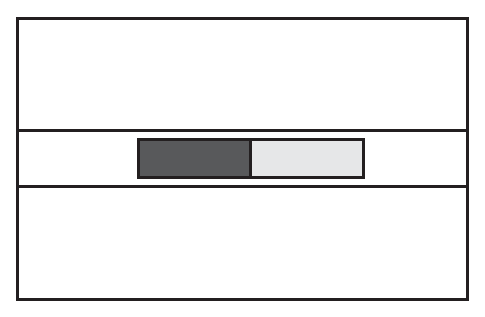
\includegraphics[scale=0.6]{06_Magnetism/magnet1.eps}&\hspace*{5mm}&
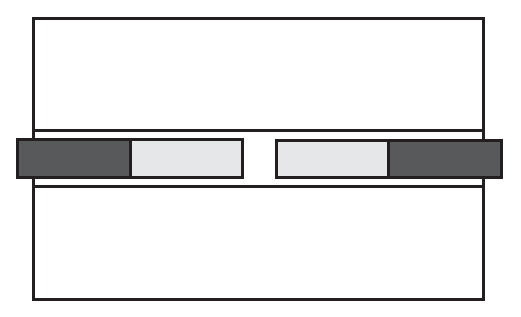
\includegraphics[scale=0.6]{06_Magnetism/magnet2.eps}
\end{tabular}
\end{center}

%\bigskip
%
%\subjikken{}
%
%地磁気の観察をしてみましょう。建物の周りの地磁気を観測し、実際の南
%北との差を調べ、その理由について考察しましょう。

%\bigskip
%\newpage


\subjikken{磁気カード上の磁場の観察}

図書カード、コピーカード、バスカードや電車の切符等にも磁性体が使わ
れています。カードのどこに磁性体がぬってあるか使用済みのカードを
磁界観察シートを使って調べてみましょう。 

\bigskip


\subjikken{磁石の種類による磁力の違い}

テスラメータを使って、アルニコ磁石、ネオジム磁石などの磁力の強さ(磁束密度)を測定して比較してみましょう。
測定する場所や磁石をつなげた時で磁束密度はどのように変化するでしょうか。

%\bigskip
\newpage

\subjikken{ヒステリシス曲線の測定}

\begin{enumerate}

\item 電磁石コイル、安定電源装置、直流電流計($\sim$5[A])を配線します。

\item 電磁石コイルの中に鉄心を入れ、鉄心の先端にテスラメータをセロハンテープで固定します。

\item 「電圧調整(粗・微)」つまみを中央、「電流調整 (粗・微)」を最小にした状態で、直流安定化電源装置の電源を入れます。

\item 電流を0.5[A]単位で5[A]まで増やしつつ、テスラメータの値を読み取り、記録します。同様に、電流を5[A]から0.5[A]
単位で0[A]まで減らしつつ磁束密度を記録します。

\item 電流と磁束密度の関係をグラフにし、磁場と磁化の間にどのような関係があるか考えましょう。
コイルの電流を増やした後、最後に電流をゼロにしても鉄心に磁束密度が残るのはどうしてでしょうか。

\end{enumerate}



